\section{A discrete portfolio on both kinds of task (Part 8)}\label{sec:portfolio}

\subsection{Protocol and designation}\label{sec:protocol8}

The question was whether one discrete method beats gradient-descent-trained networks both on the toy suites ($\nstar$ against the networks) and on the standard tasks (test error against MLPs). A protocol, written before any design result was seen, fixed the following (\cref{sec:discipline}):
\begin{itemize}
\item \emph{Development data:} the toy \code{designed} suite and the 5 DEV datasets only.
\item \emph{Fresh held-out sets:} \code{dlheld3} and HELDOUT2.
\item \emph{Budgets:} one network run per toy fit, and three MLP runs per real fit.
\item \emph{A designation rule.} On dev, a design ``beats GD'' if its mean $\log_2$ ratio is below 0 on both sides and it has more better than worse targets or cells. The toy score is the mean $\log_2\nstar$ ratio against the networks. The real score is the mean $\log_2(\text{error}/\min(\text{error of }\code{mlp},\text{error of }\code{mlp_l2}))$, with errors floored at 0.002. Among the designs that beat GD on dev, the primary is the one with the lowest sum of the two means.
\end{itemize}
Three builders worked independently, on dev data only, from different design angles: stagewise, unified boosting, and portfolio with stacking. Each design was frozen and run once on the full dev evaluation, and the rule was applied before any held-out run (\cref{tab:designation}). It picked \code{hyb_portfolio}, which is also best on each side separately. These dev scores are in-sample: the builders tuned on the same dev test sets.

\begin{table}[t]
\centering\footnotesize
\begin{tabular}{lccccc}
\toprule
design & toy mean $\log_2\nstar$ ratio & toy better / worse (of 21) & real mean $\log_2$ ratio & real better / worse (of 24) & sum\\
\midrule
\code{hyb_stage} & $-2.79$ & 21 / 0 & $-0.122$ & 1 / 0 & $-2.91$\\
\code{hyb_union} & $-2.52$ & 21 / 0 & $-0.127$ & 0 / 0 & $-2.65$\\
\code{hyb_portfolio} & $-2.98$ & 21 / 0 & $-0.248$ & 1 / 0 & $\mathbf{-3.23}$\\
\bottomrule
\end{tabular}
\caption{Dev scores of the three frozen Part 8 designs, recomputed from the result files before any held-out run. \code{hyb_union} has no better real cell, so it does not ``beat GD on dev''. Source: \repo{study/hybrid/PROTOCOL.md}.}
\label{tab:designation}
\end{table}

\subsection{The primary design}\label{sec:design}

\code{hyb_portfolio} is one \texttt{fit()} that dispatches by input type. Each member outputs class probabilities and has no continuous feature parameters (\cref{tab:members}).

\begin{table}[t]
\centering\footnotesize
\begin{tabularx}{\linewidth}{>{\raggedright\arraybackslash}p{2.3cm}>{\raggedright\arraybackslash}X>{\raggedright\arraybackslash}p{3.3cm}}
\toprule
member & what it is & when it runs\\
\midrule
\code{dfg}, \code{dfg_forced} & DFG v1.1 unchanged (\cref{sec:dfg}); \code{dfg_forced} is its small-$n$ variant ($n\le512$) & only if there are 2 classes and every column is binary or categorical ($\le256$ bits)\\
\code{gbt} & LightGBM \cite{ke2017lightgbm}: 100 rounds, learning rate 0.1, 31 leaves & always\\
\code{et} & ExtraTrees \cite{geurts2006extremely}: 100 trees; out-of-bag probabilities serve as out-of-fold predictions & always\\
\code{knn_<metric>_<k>} & $k$-nearest-neighbour vote fractions, $k\in\{1,3,9,27\}$, under the MLP's encoding and under one common scale; leave-one-out votes serve as out-of-fold predictions & always (the common-scale metric when column scales differ)\\
\code{lin_<C>} & multinomial L2 logistic regression, $C\in\{0.05,1\}$ (only $C=1$ above $n=10000$) & always\\
\bottomrule
\end{tabularx}
\caption{Members of \code{hyb_portfolio}. On the 22 held-out real datasets other than mushroom, the design is by construction a stack of LightGBM, ExtraTrees, up to 8 kNN members and 1--2 logistic regressions.}
\label{tab:members}
\end{table}

\paragraph{Stacking} \cite{wolpert1992stacked}. Let $L_m$ be member $m$'s out-of-fold log-probabilities on a stacking set. The score is $s_c(x)=b_c+\sum_m w_m L_m(x)_c$ with $w\ge0$, fitted by L2-penalized multinomial log-loss, which is convex.
\begin{itemize}
\item \emph{Stacking set:} 10-fold cross-validation for $n\le500$, 5-fold for $n\le3000$, and above that one stratified holdout of $\min(n/5,6000)$ points.
\item \emph{Refits:} DFG, LightGBM and logistic regression are refitted on all $n$.
\end{itemize}

\paragraph{Budget split.} DFG's out-of-fold fits share 35\% of the budget, and its final fit(s) get at most 50\%. Every other member is skipped if its projected cost exceeds 90--95\% of the budget; this never triggered on dev.

\paragraph{Large inputs.} When $n\cdot d>10^7$ (MNIST and Fashion-MNIST at $n\ge30000$), the design switches to:
\begin{itemize}
\item float32 encodings;
\item LightGBM with row subsampling 0.5 and column subsampling 0.25;
\item no LightGBM refit.
\end{itemize}
These settings came from synthetic timing runs and had never run on real data before the held-out evaluation.

\subsection{Toy results}\label{sec:toyresults}

\begin{table}[t]
\centering
\resizebox{\linewidth}{!}{\small\setlength{\tabcolsep}{3.5pt}\begin{tabular}{lrrrrrrrrrr}
\toprule
target & portfolio & \hd{DFG\\alone} & \hd{without\\DFG} & \texttt{lin} & \texttt{hgb} & \texttt{nets} & \texttt{nets\_wd} & \texttt{nets\_cewd} & \texttt{nets\_best} & \hd{$\log_2$ ratio to\\\texttt{nets\_best}}\\
\midrule
cnf3 & 146 & 213 & 130 & never & 164 & 489 & 371 & 361 & 361 & $-1.31$\\
dlist8 & 24 & 31 & 26 & 91 & 61 & 104 & 90 & 108 & 90 & $-1.91$\\
h3rf0 & 46 & 51 & 48 & 112 & 60 & 109 & 96 & 113 & 96 & $-1.06$\\
h3rf1 & 60 & 56 & 80 & 101 & 63 & 123 & 101 & 121 & 101 & $-0.75$\\
mixmaj & 96 & 109 & 341 & never & 368 & 507 & 361 & 326 & 326 & $-1.76$\\
mux11 & 523 & 826 & 521 & never & 573 & 1527 & 1245 & 1699 & 1245 & $-1.25$\\
par3or & 62 & 61 & 7531 & never & 2009 & 1050 & 725 & 842 & 725 & $-3.54$\\
poly4 & 177 & 177 & never & never & never & 10199 & 6609 & 2745 & 2745 & $-3.95$\\
sym9 & 1229 & 1220 & 7113 & never & 7845 & 787 & 563 & 350 & 350 & $+1.81$\\
thrint & 149 & 167 & 142 & 137 & 243 & 546 & 267 & 190 & 190 & $-0.36$\\
\bottomrule
\end{tabular}
}
\caption{The fresh toy suite \code{dlheld3}: $\nstar$ per target, inputs permuted per fit \status{Numerical}. ``portfolio'' is \code{hyb_portfolio}; ``DFG alone'' and ``w/o DFG'' are the post-hoc ablations of \cref{sec:attribution}. The last column is $\log_2$ of the portfolio's $\nstar$ over \code{nets_best}'s, from unrounded values. Generated by \texttt{make\_tables.py} from \repo{study/hybrid/results/}; the values agree with \repo{study/hybrid/RESULTS.md}.}
\label{tab:dlheld3}
\end{table}

\begin{table}[t]
\centering\footnotesize\setlength{\tabcolsep}{4pt}
\begin{tabular}{lllllll}
\toprule
suite & targets & status & vs \texttt{nets} & vs \texttt{nets\_wd} & vs \texttt{nets\_best} & \texttt{lin} vs \texttt{nets\_best}\\
\midrule
\texttt{designed} & 21 & development & $-2.97$ (21/0) & $-2.32$ (21/0) & $-2.32$ (21/0) & $-0.56$ (5/14)\\
\texttt{random} & 20 & DFG development data & $-2.89$ (20/0) & $-2.24$ (20/0) & $-2.24$ (20/0) & $-0.05$ (2/16)\\
\texttt{dlheld} & 12 & post hoc for DFG & $-2.24$ (12/0) & $-1.75$ (10/0) & $-1.75$ (10/0) & $-0.36$ (2/9)\\
\texttt{dlheld2} & 7 & blind for DFG v1.1, used once & $-2.17$ (7/0) & $-1.54$ (6/0) & $-1.54$ (6/0) & $-0.76$ (2/4)\\
\texttt{dlheld3} & 10 & \textbf{fresh} & $-2.12$ (9/1) & $-1.67$ (9/1) & $-1.41$ (9/1) & $-0.06$ (1/6)\\
\bottomrule
\end{tabular}

\caption{\code{hyb_portfolio} (inputs permuted) on all five toy suites: mean $\log_2\nstar$ ratio against each network reference, with the number of targets clearly better / clearly worse in brackets \status{Numerical}. The last column shows logistic regression alone against \code{nets_best}; its ``worse'' counts include every target it never learns. Outside \code{dlheld3}, \code{nets_best} equals \code{nets_wd}.}
\label{tab:toysuites}
\end{table}

\begin{figure}[t]
\centering
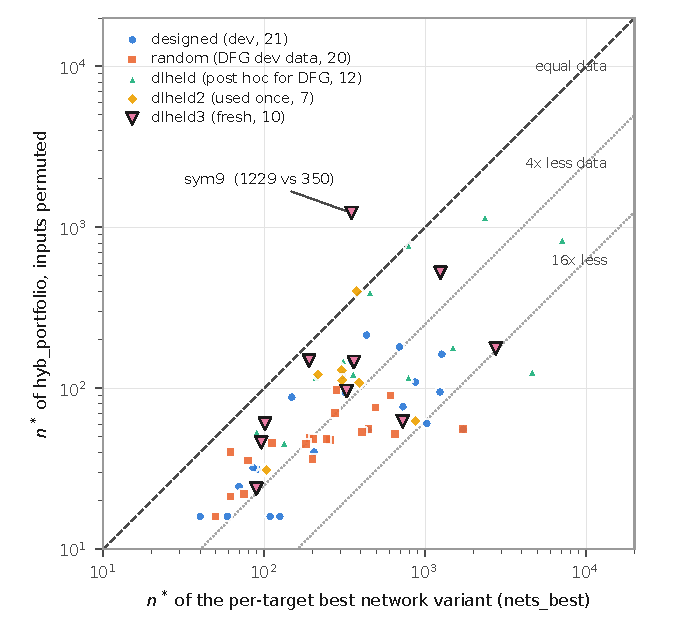
\includegraphics[width=0.72\linewidth]{figures/fig_toy_portfolio.pdf}
\caption{\code{hyb_portfolio}'s $\nstar$ (inputs permuted per fit) against the per-target best network variant, for all 70 targets of the five toy suites. Each suite has its own marker shape and colour, and the fresh suite \code{dlheld3} is outlined. The dashed line is equal data; the dotted lines mark 4 and 16 times less. The one target above the diagonal is sym9.}
\label{fig:toy}
\end{figure}

\paragraph{The fresh suite} (\cref{tab:dlheld3}). \code{hyb_portfolio} needs clearly less data than \code{nets_best} on 9 of 10 targets \status{Numerical}.
\begin{itemize}
\item \emph{Against \code{nets_best}:} mean $\log_2$ ratio $-1.41$, about $2.7\times$ less data.
\item \emph{Against single configurations:} $-1.55$ against \code{nets_cewd}, $-1.67$ against \code{nets_wd} and $-2.12$ against \code{nets}.
\item \emph{The one loss:} sym9.
\item \emph{Input order and compute.} The natural-order run is nearly identical ($-1.42$ against \code{nets_best}), and the largest fit uses 0.66 of one network run.
\item \emph{Without the linear-model win.} Excluding the target on which logistic regression alone already wins (thrint), the portfolio is clearly better on 8 and clearly worse on 1 of 9, mean $-1.52$.
\end{itemize}
The margins differ by kind of target.
\begin{itemize}
\item \textbf{Targets with parity components}, which trees and linear models do not see.
  \begin{itemize}
  \item par3or: $-3.54$. \code{hgb} needs 2009 samples, and \code{lin} never reaches 10\% error.
  \item poly4: $-3.95$. Neither \code{hgb} nor \code{lin} ever learns it.
  \item mixmaj: $-1.76$.
  \end{itemize}
  These margins survive every network variant, and they are DFG's (\cref{sec:attribution}).
\item \textbf{mux11 and cnf3} ($-1.25$, $-1.31$). The trees can carry these.
\item \textbf{Threshold, decision-list and random-formula targets} (thrint, dlist8, h3rf0, h3rf1). The margins are constant factors, $-0.36$ to $-1.91$ in $\log_2$. thrint's shrinks most with the regularized networks, from $-1.88$ against \code{nets} to $-0.36$ against \code{nets_cewd}.
\end{itemize}

\paragraph{sym9, the one loss.} The portfolio's seed-mean test error on sym9 is 0.39 at $n=256$, 0.20 at 512, 0.13 at 1024 and 0.014 at 2048, so $\nstar=1229$. The logistic-loss, weight-decayed networks reach 10\% at about 350. DFG alone gets 1220 and the portfolio without DFG 7113, so the loss is DFG's. The secondary design \code{hyb_stage} (591) comes closer. A reading, not tested in Part 8 \status{Heuristic}:
\begin{itemize}
\item sym9 depends on the inputs only through $x_1+\dots+x_9$, so a network can represent it with units on the single direction $(1,\dots,1)$.
\item Its Fourier weight is spread over many characters of degrees 2, 4, 6 and 8, with equal coefficients within each degree. A character search pays for each of them separately.
\end{itemize}
Part 9 tests this reading (\cref{sec:part9}).

\paragraph{The other suites} (\cref{tab:toysuites}, \cref{fig:toy}). These are development data, or not blind for DFG. On their 60 targets the portfolio is clearly better than every network reference on 57 and tied on 3:
\begin{itemize}
\item inter2, 394 against 454, and majxor, 771 against 792, on \code{dlheld};
\item sym8, 401 against 377, on \code{dlheld2}.
\end{itemize}
sym8 is the same kind of target as sym9, and the only target outside \code{dlheld3} on which the portfolio is above a network reference, inside the tie band.

\paragraph{Stronger networks.} The fairness audit's probe found that weight decay 0.1, or logistic loss plus weight decay, cuts the networks' $\nstar$ by about $2\times$ at the same compute. In the full runs the largest cut is $3.7\times$, on poly4 (10199 to 2745).
\begin{itemize}
\item \emph{Margin shrink.} Against \code{nets_best} the portfolio's suite-mean margins shrink, relative to \code{nets}, by 0.65, 0.66, 0.49, 0.63 and 0.72 in $\log_2$ on the five suites.
\item \emph{Which targets.} The shrink is spread over every kind of target. The largest per-target shrinks are on \code{dlheld3}: poly4 by 1.9, thrint by 1.5 and sym9 by 1.2.
\item \emph{Signs.} The per-target sign is the same against every reference: negative on 9 targets, positive on sym9. sym9 is already $+0.64$ against the unregularized \code{nets} (787).
\item \emph{What \code{nets_best} is.} On \code{dlheld3} it is a hindsight minimum that no single configuration achieves: \code{nets_cewd} is best on 5 targets and \code{nets_wd} on 5, and \code{nets_cewd} is worse than plain \code{nets} on mux11, dlist8 and h3rf0.
\end{itemize}

\paragraph{Input permutation.} The first held-out toy runs used the natural input order. All three designs break exact ties toward low column indices, through DFG's enumeration order and LightGBM's split choice, so every held-out toy suite was re-run with the columns permuted per fit. That run is the headline.
\begin{itemize}
\item \emph{Suite means:} they change by 0.01--0.04 in $\log_2$ against \code{nets}.
\item \emph{Single targets:} they change by up to 0.64, in both directions. The largest is par5 on \code{dlheld}: 539 in natural order, 839 permuted.
\end{itemize}

\paragraph{What logistic regression alone does}\label{sec:lin} \status{Numerical}. On halfspace-like targets the portfolio's win over the networks is a linear-model win.
\begin{itemize}
\item \code{lin} alone is clearly better than \code{nets_best} on:
  \begin{itemize}
  \item 5 designed targets: dict, maj3, maj9, rand2, thr10;
  \item 2 random formulas;
  \item maj15 and thr30 on \code{dlheld}, maj21 and thr20 on \code{dlheld2}, and thrint on \code{dlheld3}.
  \end{itemize}
\item On those halfspaces the portfolio is at \code{lin}'s level or slightly above it: for example maj15 118 against 110, thr20 130 against 117, thrint 149 against 137.
\item Excluding the targets \code{lin} wins makes the portfolio's mean margins larger, not smaller.
\end{itemize}

\subsection{Tabular results}\label{sec:tabular}

\begin{table}[t]
\centering\footnotesize\setlength{\tabcolsep}{3.5pt}
\begin{tabular}{lcccc}
\toprule
split (datasets, cells) & vs \code{mlp} & vs \code{mlp_reg} & vs \code{mlp_strong} & vs \code{mlp_best}\\
\midrule
\textbf{HELDOUT2, fresh} (10, 53) & $-0.44$; 15/36/2; 9 of 10 (0.021) & $-0.27$; 16/35/2; 8 (0.11) & $-0.28$; 15/36/2; 8 (0.11) & $\mathbf{-0.17}$; 10/41/2; 8 (0.11)\\
Part 7 tabular (11, 59) & $-0.33$; 22/36/1; 10 of 11 (0.012) & $-0.16$; 16/40/3; 9 (0.065) & $-0.34$; 22/30/2; 10 (0.012)$^\dagger$ & $-0.11$; 12/44/3; 8 (0.23)\\
images (2, 14) & $-0.28$; 7/7/0; 2 of 2 (0.5) & $-0.14$; 2/12/0; 2 (0.5) & $+0.05$; 1/9/4; 0 (0.5) & $+0.05$; 1/9/4; 0 (0.5)\\
dev, in-sample (5, 24) & $-0.38$; 4/20/0; 5 of 5 (0.062) & $-0.27$; 3/21/0; 5 (0.062) & not run & $-0.25$; 1/23/0; 5 (0.062)\\
\addlinespace
\multicolumn{5}{l}{\emph{calibration, against \code{mlp_best}:} \code{hgb} $+0.08$ (HELDOUT2), $+0.14$ (Part 7 tabular), $+0.26$ (images); baseline \code{mlp} $+0.28$, $+0.22$, $+0.34$.}\\
\bottomrule
\end{tabular}
\caption{\code{hyb_portfolio} on standard tasks \status{Numerical}. Each entry gives the mean $\log_2(\text{error}/\text{reference error})$ over cells; better / tie / worse cells; and the number of datasets with lower mean error, with the two-sided sign-test $p$ in brackets. $^\dagger$\code{mlp_strong} was run on the Part 7 tabular set only at $n\le10000$ (54 of 59 cells), and it is weak on pendigits and ring, so \code{mlp_best} is the stricter reference there. Source: \repo{study/hybrid/RESULTS.md}.}
\label{tab:real}
\end{table}

\begin{figure}[t]
\centering
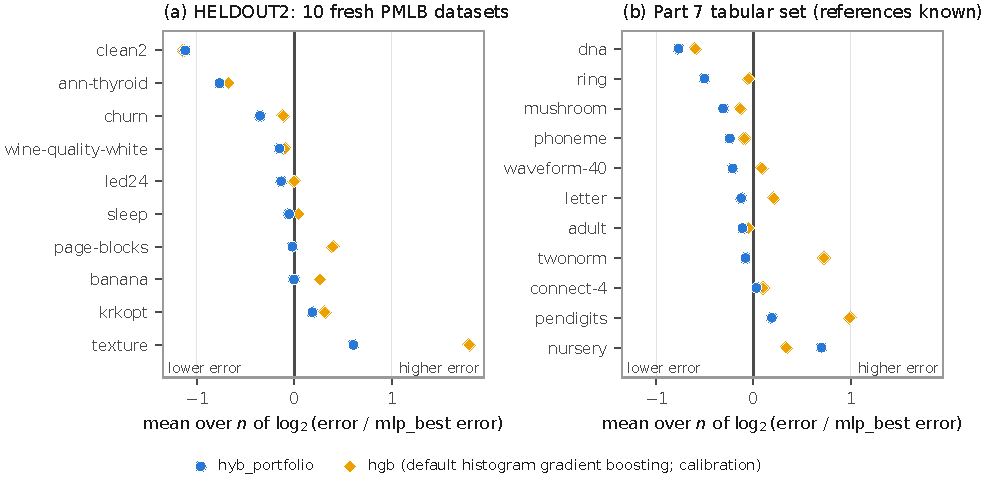
\includegraphics[width=\linewidth]{figures/fig_tabular.pdf}
\caption{Per-dataset mean over $n$ of $\log_2(\text{error}/\text{\code{mlp_best} error})$, for \code{hyb_portfolio} and, for calibration, default \code{hgb}. Negative is better than the hindsight-best MLP. (a) The fresh HELDOUT2 set. (b) The Part 7 tabular set, whose MLP references the Part 8 builders had seen. Computed with \texttt{compare\_hybrid.py}'s cell rule from the result files.}
\label{fig:tabular}
\end{figure}

\paragraph{The fresh datasets} (\cref{tab:real}, \cref{fig:tabular}) \status{Numerical}.
\begin{itemize}
\item \emph{Against \code{mlp_best}:} the mean error is lower on 8 of 10 datasets (sign test $p=0.11$, not significant). The mean $\log_2$ error ratio is $-0.17$, a geometric-mean error about 11\% lower, with 10 of 53 cells better and 2 worse.
\item \emph{Against single references} the margins are larger: $-0.28$ against the strong MLP ensemble, which has twice the budget, and $-0.32$ against one network of that recipe (15 better, 2 worse). The sign test is 8 of 10 against all three.
\item \emph{How strong the 8 of 10 is.} Three of the 8 datasets are within about $\pm0.05$: page\_blocks, banana and sleep. The large margins are on ann\_thyroid (4 resolved cells), churn (2) and clean2. clean2's $-1.12$ comes mostly from $n\le300$ and has 1 resolved cell.
\item \emph{Losses.} The portfolio loses on texture (11 classes, 40 continuous inputs): its error is higher at every $n$ ($+0.61$), but no cell resolves, since errors are below 1.6\% from $n=1000$. Logistic regression alone matches the stack there, and the trees are 2--3$\times$ worse. It also loses on krkopt (18 classes, a chess endgame), resolved at $n\ge10000$: 0.2037 against \code{mlp_strong}'s 0.1333 at full $n$.
\end{itemize}

\paragraph{The Part 7 tabular set}, whose references the designers had read.
\begin{itemize}
\item \emph{Overall:} $-0.11$ against \code{mlp_best}, lower mean error on 8 of 11 datasets ($p=0.23$).
\item \emph{Largest wins:} dna ($-0.77$, 3 resolved cells), ring ($-0.50$), mushroom ($-0.31$) and phoneme ($-0.24$).
\item \emph{Losses:} nursery ($+0.70$, worse at $n=1000$ and 3000), pendigits ($+0.19$, none resolved) and connect\_4 ($+0.03$, worse at full $n$: 0.1566 against 0.1412).
\end{itemize}

\paragraph{Calibration.} Default \code{hgb} alone does not beat the MLPs on average ($+0.08$ on HELDOUT2, $+0.14$ on the Part 7 set). The baseline \code{mlp} trails \code{mlp_best} by $+0.28$ and $+0.22$, which shows how much of the margin over \code{mlp} is the baseline's weakness. These numbers agree with the tabular-learning literature: tree ensembles and stacking tend to beat plain MLPs on medium-sized tabular data \cite{grinsztajn2022tree,shwartzziv2022tabular}, and careful regularization of the MLP narrows the gap \cite{kadra2021welltuned,gorishniy2021revisiting}.

\subsection{Images}\label{sec:images}

\begin{figure}[t]
\centering
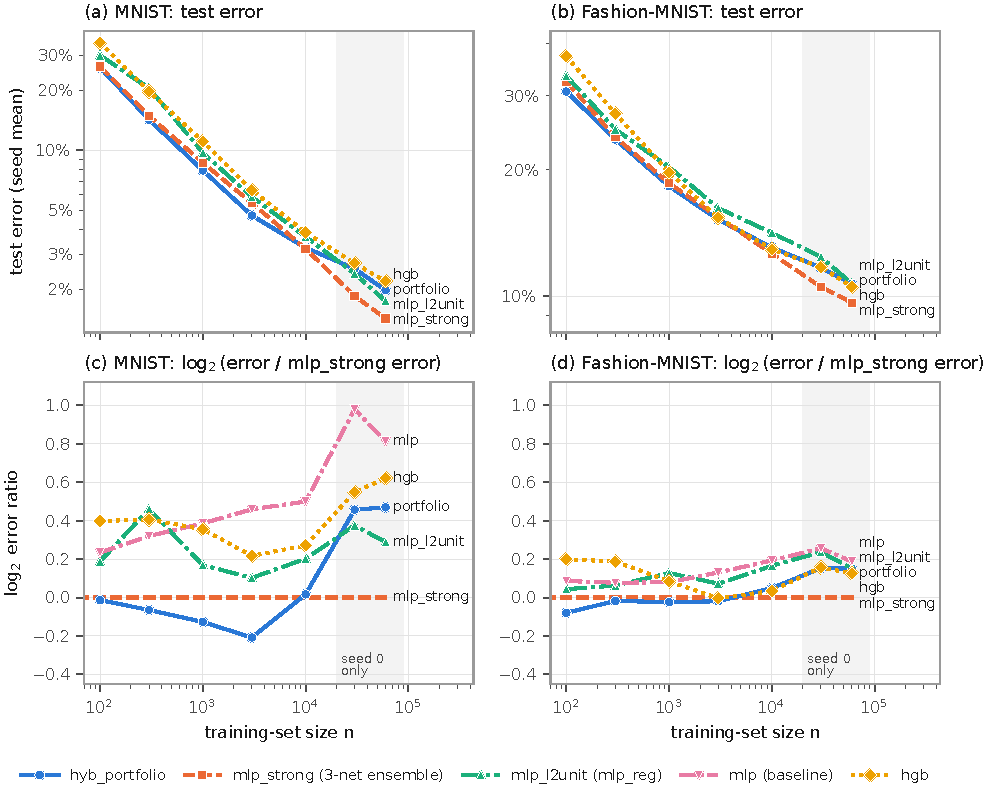
\includegraphics[width=\linewidth]{figures/fig_images.pdf}
\caption{MNIST and Fashion-MNIST. (a, b) Seed-mean test error against training-set size for \code{hyb_portfolio}, the strong MLP ensemble \code{mlp_strong} (twice the FLOP budget), the regularized MLP \code{mlp_l2unit} and default \code{hgb}. (c, d) $\log_2$ of each learner's error over \code{mlp_strong}'s, adding the baseline \code{mlp}; the dashed line at 0 is \code{mlp_strong}. Shaded: $n\ge30000$, where the portfolio and \code{mlp_strong} are seed 0 only. There is no fresh image set, and the Part 8 builders had seen the MLP references.}
\label{fig:images}
\end{figure}

\begin{table}[t]
\centering\footnotesize\setlength{\tabcolsep}{4pt}
\begin{tabular}{lrcccccc}
\toprule
dataset & $n$ & \code{mlp} & \code{mlp_l2unit} & \code{mlp_strong} & \code{mlp_strong1} & \code{hyb_portfolio} & \code{hgb}\\
\midrule
MNIST & 300 & 0.1862 & 0.2052 & 0.1492 & 0.1528 & \textbf{0.1426} & 0.1977\\
 & 3000 & 0.0747 & 0.0583 & 0.0543 & 0.0556 & \textbf{0.0470} & 0.0631\\
 & 10000 & 0.0452 & 0.0368 & \textbf{0.0320} & 0.0327 & 0.0324 & 0.0386\\
 & 30000 & 0.0365 & 0.0240 & \textbf{0.0185} & 0.0192 & 0.0254 & 0.0271\\
 & 60000 & 0.0251 & 0.0175 & \textbf{0.0143} & 0.0161 & 0.0198 & 0.0220\\
\addlinespace
Fashion-MNIST & 300 & 0.2523 & 0.2498 & 0.2392 & 0.2449 & \textbf{0.2363} & 0.2724\\
 & 3000 & 0.1690 & 0.1623 & 0.1544 & 0.1571 & \textbf{0.1523} & 0.1540\\
 & 10000 & 0.1445 & 0.1417 & \textbf{0.1264} & 0.1305 & 0.1307 & 0.1294\\
 & 30000 & 0.1258 & 0.1241 & \textbf{0.1053} & 0.1131 & 0.1171 & 0.1174\\
 & 60000 & 0.1100 & 0.1073 & \textbf{0.0966} & 0.0992 & 0.1072 & 0.1054\\
\bottomrule
\end{tabular}
\caption{Seed-mean test error on images (selected $n$; all $n$ in \cref{fig:images}) \status{Numerical}. At $n\ge30000$, every column except \code{mlp}, \code{mlp_l2unit} and \code{hgb} is seed 0 only. Source: \repo{study/hybrid/HYBRID.md}, \S4.4.}
\label{tab:images}
\end{table}

There is no fresh image set, and the designers had seen the references, so this is the weakest evidence in Part 8 (\cref{tab:images}, \cref{fig:images}) \status{Numerical}.
\begin{itemize}
\item \emph{$n\le3000$.} The portfolio's error is below every MLP variant's in all 8 cells, by about 1--13\% relative. Against \code{mlp_best}, which is \code{mlp_strong} at every image $n$, only MNIST $n=3000$ resolves as better: 4.70\% against 5.43\%.
\item \emph{$n=10000$.} About equal: 3.24\% against 3.20\% on MNIST, and 13.07\% against 12.64\% on Fashion-MNIST.
\item \emph{$n=30000$ and 60000.} The strong MLP ensemble is clearly better in all four cells. At 60000 it has 1.43\% against the portfolio's 1.98\% on MNIST, and 9.66\% against 10.72\% on Fashion-MNIST.
\item \emph{One network of the strong recipe.} \code{mlp_strong1} also has lower error than the portfolio at $n\ge30000$ on both datasets, but this resolves only at MNIST $n=30000$ (1.92\% against 2.54\%).
\item \emph{Default \code{hgb}.} On Fashion-MNIST at large $n$ the portfolio is no better than \code{hgb}: 10.72\% against 10.54\% at 60000.
\end{itemize}
The stronger reference reverses the large-$n$ cells, which the fairness audit had flagged as the ones most likely to flip. With enough data, a well-regularized MLP's learned continuous directions beat prototype memory and axis-aligned trees, the same reading as in \cref{sec:whyfail} \status{Heuristic}.

\subsection{What carries which result}\label{sec:attribution}

\begin{figure}[t]
\centering
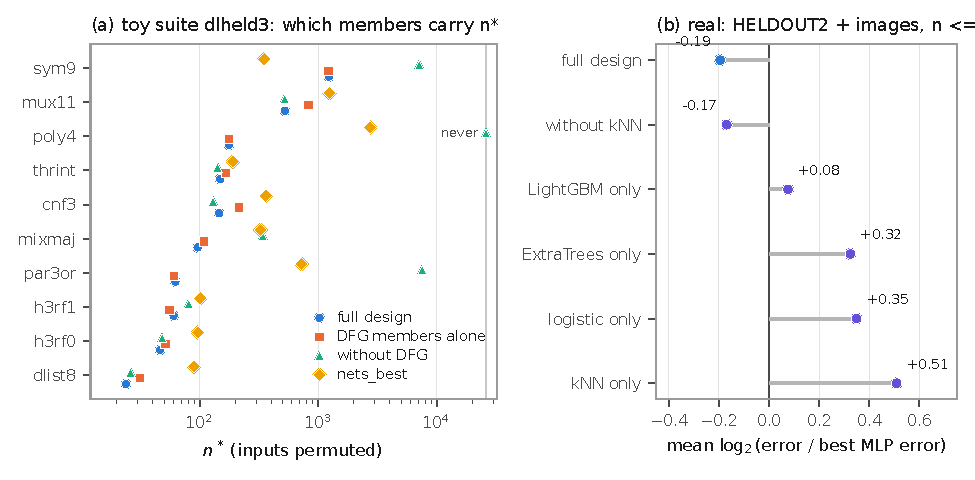
\includegraphics[width=\linewidth]{figures/fig_ablations.pdf}
\caption{Post-hoc attribution ablations of the frozen \code{hyb_portfolio}, run with its \texttt{members} argument after the held-out results. (a) $\nstar$ on \code{dlheld3} (inputs permuted) for the full design, the DFG members alone (stacked), all members except DFG, and \code{nets_best}. (b) Mean $\log_2(\text{error}/\text{best MLP error})$ over 48 cells (HELDOUT2 and the two image sets, $n\le3000$, seeds 0--1), for the full design and for single member families. Here ``best MLP'' is the per-cell best seed-mean over seeds 0--1.}
\label{fig:ablations}
\end{figure}

These ablations are post hoc and not part of the held-out test (\cref{fig:ablations}) \status{Numerical}.

\paragraph{Toy.}
\begin{itemize}
\item \emph{Without DFG}, the design fails on the parity-like targets: par3or needs 7531 samples (62 with DFG), mixmaj 341 (96), sym9 7113 (1229), and poly4 is never learned. Its mean on \code{dlheld3} becomes $+0.17$ against \code{nets_best} (6 clearly better, 3 clearly worse). It still wins clearly on 6 of 10 fresh targets, with the trees carrying cnf3 (130) and mux11 (521). On \code{designed} it falls from $-2.32$ to $-0.63$ and never learns par4.
\item \emph{DFG alone} (its two members, stacked) is close to the full design: $-1.21$ on \code{dlheld3} and $-2.13$ on \code{designed}. The other members add on AND, OR and threshold structure: cnf3 213 against 146, mux11 826 against 523, and on \code{designed} and3 74 against 25.
\end{itemize}

\paragraph{Real.}
\begin{itemize}
\item \emph{No single member family matches the stack.} The best, LightGBM alone, is $+0.08$, behind the MLPs on average, while the full design is $-0.19$. The gain comes from combining members.
\item \emph{Different members carry different datasets.}
  \begin{itemize}
  \item trees: churn, ann\_thyroid and clean2;
  \item kNN: banana;
  \item logistic regression: texture;
  \item ExtraTrees and logistic regression: led24 and sleep.
  \end{itemize}
\item \emph{kNN matters on MNIST.} Without it, MNIST errors at $n=100$, 300, 1000 and 3000 rise from 0.2563, 0.1458, 0.0779 and 0.0476 to 0.2687, 0.1609, 0.0913 and 0.0606, above the best MLP.
\item \emph{DFG runs on no HELDOUT2 dataset and on neither image set.} The spectral block and the oracle best single member per cell were not ablated.
\end{itemize}

\paragraph{Reading} \status{Heuristic}. The toy result is Part 6's mechanism: exhaustive enumeration pays about $\ln N$ samples per character, where gradient descent on a generic MLP pays much more on targets without low-degree marginal signal. The classical members add constant factors on dense targets. The tabular result restates known facts about tree ensembles and stacking \cite{grinsztajn2022tree,erickson2020autogluon}.

\subsection{Compute and prediction cost}\label{sec:compute8}

\begin{itemize}
\item \textbf{Fit FLOPs}, by the learner's own counts:
  \begin{itemize}
  \item toy: at most 0.75 of one network run (on \code{dlheld});
  \item real: at most 0.24 of the budget on the Part 7 tabular set, 0.09 on HELDOUT2 and 0.54 on images.
  \end{itemize}
\item \textbf{Correction.} The compute audit found the LightGBM charge off by $0.05$--$1.7\times$ against an algorithmic count that tracks CPU time. With its correction, the largest image fit is about 0.74 of the budget (range 0.58--0.90, Fashion-MNIST $n=3000$).
\item \textbf{Not a bound.} The toy compute is bounded by measurement, not by construction: the audit's worst-case bound is about 1.1.
\item \textbf{Prediction and CPU time.} Prediction is not counted for any learner, but it is not cheap here. The kNN members scan all $n$ training points: at $n=60000$ that is $1.9\times10^8$ FLOPs per query, about $350\times$ an MLP's. CPU time is also far larger on images: about 8 CPU-minutes for a Fashion-MNIST fit at $n=3000$, against an estimated 25--40\,s for the three MLP runs that the budget corresponds to.
\end{itemize}
The portfolio's real-data wins are therefore not bought with more FLOPs than the references, but they are bought with more CPU time on images and far more prediction cost (\cref{app:compute}).

\subsection{The secondary designs}\label{sec:secondary}

\begin{table}[t]
\centering\footnotesize\setlength{\tabcolsep}{4pt}
\begin{tabular}{lll}
\toprule
 & \code{hyb_stage} & \code{hyb_union}\\
\midrule
toy \code{designed}, permuted, vs \code{nets_best} & $-2.11$ (21/0) & $-1.85$ (21/0)\\
toy \code{dlheld3}, permuted, vs \code{nets_best} & $-1.60$ (9/1; sym9 591) & $-0.71$ (8/1; sym9 3151)\\
HELDOUT2 vs \code{mlp_strong} & $-0.16$; 10/40/3; 7 of 10 (0.34) & $-0.10$; 9/42/2; 6 of 10 (0.75)\\
HELDOUT2 vs \code{mlp_best} & $-0.05$; 6/40/7; 6 of 10 (0.75) & $+0.01$; 2/49/2; 6 of 10 (0.75)\\
Part 7 tabular vs \code{mlp_best} & $+0.02$; 6/46/7; 7 of 11 (0.55) & not run\\
images vs \code{mlp_strong} & $+0.18$; 0/8/6 & $+0.13$; 0/10/4\\
\bottomrule
\end{tabular}
\caption{The two secondary designs, frozen and evaluated with scope cuts \status{Numerical}. Entries as in \cref{tab:toysuites,tab:real}.}
\label{tab:secondary}
\end{table}

\begin{itemize}
\item \textbf{\code{hyb_stage}} runs stagewise.
  \begin{itemize}
  \item \emph{Design.} A multi-class port of DFG's search (characters on binary, one-hot and thermometer bits, linear and spectral blocks, kNN votes) is read out by penalized logistic regression. LightGBM is then fitted on its margins, and a stage set is chosen by cross-validation.
  \item \emph{Where it beats the primary.} On \code{dlheld3} ($-1.60$ against $-1.41$; sym9 591 against 1229), and at full $n$ on krkopt (0.1622 against 0.2037) and connect\_4 (0.1360 against 0.1566).
  \item \emph{Where it is worse.} On texture and on images.
  \end{itemize}
\item \textbf{\code{hyb_union}} is unified boosting over trees, Fourier characters, linear steps and honest blocks, with a 480\,s wall-clock stop.
  \begin{itemize}
  \item It is weakest on the toy suite, and about level with \code{mlp_best} on HELDOUT2.
  \item Its parity family is essentially idle on real data.
  \item Its large-$n$ results depend on machine load.
  \end{itemize}
\end{itemize}
Neither secondary design would change the overall answer (\cref{tab:secondary}).

\subsection{What ``discrete'' means, and the honest claim}\label{sec:discreteness}

\paragraph{Discreteness.} What the hypothesis is made of:
\begin{itemize}
\item a weighted sum of tree cells, Fourier characters, nearest-neighbour votes, the raw inputs, and DFG's spectral features;
\item fitted continuously: only convex readouts and stacking weights, plus boosting's Newton leaf values on fixed partitions;
\item no neural network, and no gradient descent on a continuous feature parameter.
\end{itemize}
Some components are borderline.
\begin{itemize}
\item \emph{Gradient boosting} is functional gradient descent over trees. The line between this method and the networks is ``no continuous feature parameters'', not ``no gradients''.
\item \emph{kNN votes} are memory under a fixed Euclidean metric.
\item \emph{Logistic regression} on continuous inputs is a linear background, not a discrete feature.
\item \emph{DFG's spectral block} produces $(u\cdot x)^2$ with $u$ a continuous eigenvector of a residual-weighted second-moment matrix: one closed-form step of continuous feature learning. In the primary design it acts only through DFG, so only on Boolean two-class inputs. It was not ablated.
\end{itemize}

\paragraph{The claim, worded as the evidence allows.} One learner, which never trains a neural network or any continuous feature parameter:
\begin{itemize}
\item needs clearly less data than the study's gradient-descent-trained networks (width-128 MLPs, 20000 Adam steps, three loss and regularization settings) on 9 of 10 fresh toy Boolean targets, and clearly more on one symmetric function;
\item has lower error on average than the hindsight-best MLP on 10 fresh tabular datasets, which is not significant (8 of 10, $p=0.11$);
\item on MNIST and Fashion-MNIST, is slightly below every MLP at $n\le3000$ (resolved in 1 of 8 cells), level at $n=10000$, and clearly above a regularized ensemble of three MLPs at $n\ge30000$.
\end{itemize}
It is an AutoML-style portfolio, Part 6's character search plus a standard stack, and its two halves are carried by different parts: the toy suites by the character search, and real data by the classical stack. It does not unify the two kinds of structure.
